\chapter{Components and Applications}
\label{cha:toolsandcomponents}

\GrG\ is combined from two groups of components:
The first consists of the compiler \texttt{grgen} and some runtime libraries, which offer the basic functionality of the system;
the compiler transforms specifications of declarative graph rewrite rules into highly efficient .NET-assemblies.
With one of these libraries, you can optionally enable automatic graph persistence.
The second consists of the interactive command line \texttt{(G)GrShell} and the graph viewers \texttt{yComp} and MSAGL with some further runtime libraries,
which offer a rapid prototyping environment supporting graphical and stepwise debugging of rules that are controlled by sequences.
These functionalitie are also available on API level, you can add graph visualization, stepwise sequence/rule debugging, or even shell scripting to your end user app.

Figure~\ref{figcomponentsapps} gives an overview of the \GrG\ system components and the applications.
In the following, we are going to visit them component by component.

\begin{figure}[htbp]
  \centering
  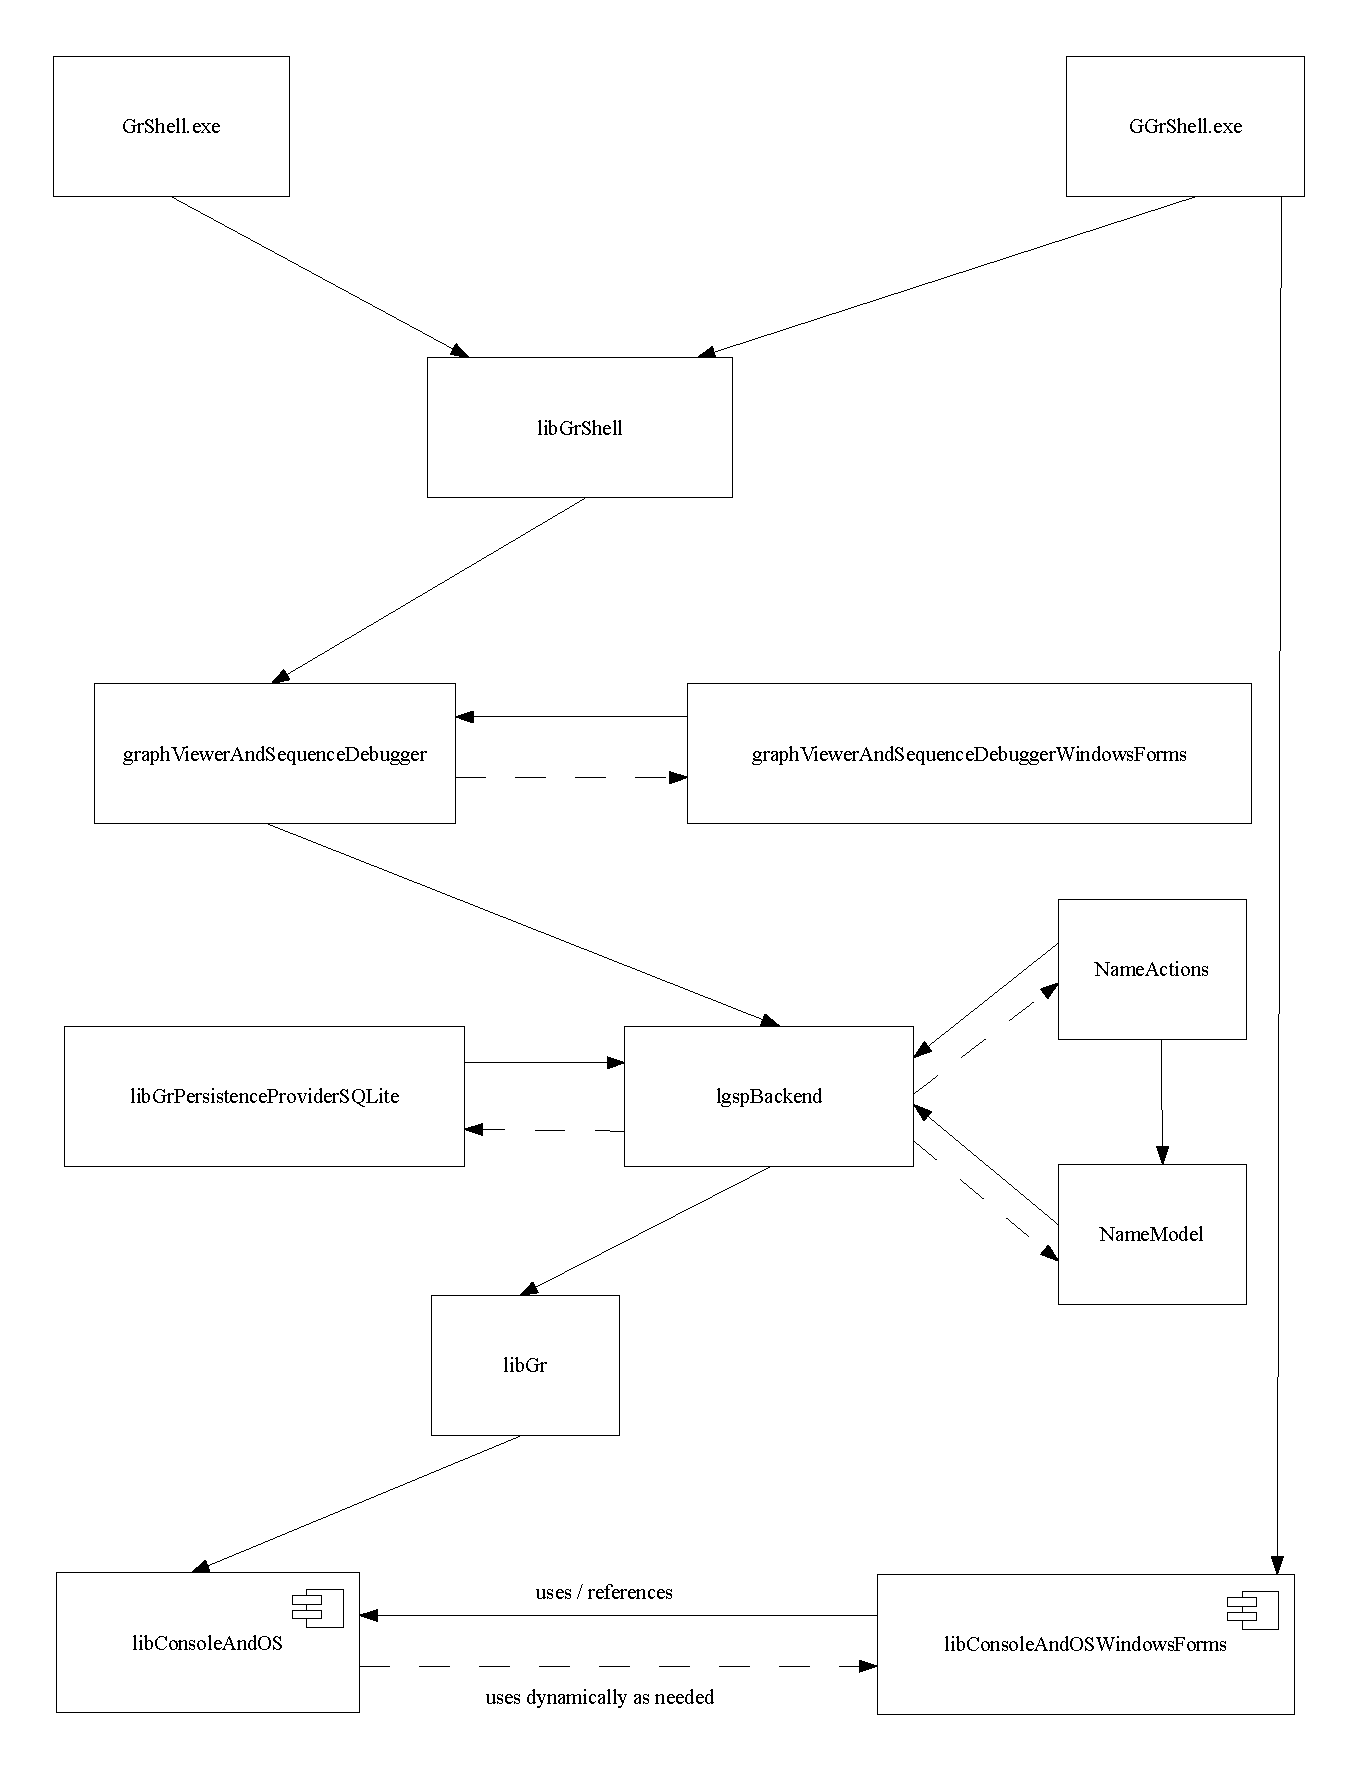
\includegraphics[width=\textwidth]{fig/ComponentsAndApps}
  \caption{\GrG\ system components and applications (draft)}
  \label{figcomponentsapps}
\end{figure}


%%%%%%%%%%%%%%%%%%%%%%%%%%%%%%%%%%%%%%%%%%%%%%%%%%%%%%%%%%%%%%%%%%%%%%%%%%%%%%%%%%%%%%%%%%%%%%%%
%\section{The Tools}

The programs and libraries of \GrG\ are open source licensed under \indexed{LGPL}\cite{LGPL3}.
Notice that the \yComp\ graph viewer is not a part of \GrG ; \yComp\ (cf. \url{https://pp.ipd.kit.edu/firm/yComp.html}) is closed source and ships with its own license granted by \yFiles\ for academic use --
this means above all that you are not allowed to ship it with a release of your own commercial software, in contrast to the \GrG\ libraries.
To be more specific: an academic license restricts the use of the software (\yComp) to \emph{non-commercial} purposes (research, teaching, projects, courses and application development).
Utilizing the internal \MSAGL{} based graph viewer saves you from license issues due to its permissive MIT license, but it lacks the sophistication of \yComp{}.
The persistent graph is implemented (by an internal persistence provider) utilizing the SQLite database and its ADO.NET drivers, which are in the public domain.

Executing a generated graph rewrite system requires .NET Framework\cite{NET} version 4.7.2 or mono\cite{MONO} version 5.10, or later (maybe complete packaging); compiling (and debugging with \yComp) a graph rewrite system in addition requires JAVA\cite{JAVA} version 1.8 or later. 
You find the tools in the \texttt{bin} subdirectory of your \GrG\ installation.

%-----------------------------------------------------------------------------------------------
\section{\texttt{\indexed{GrGen.exe}}} \label{grgenoptions}

\parpic[l] {
\includegraphics[width=48pt]{fig/grgen-256.png}
}
\noindent The \texttt{GrGen.exe} assembly implements the \GrG\ generator.
The \GrG\ generator parses a rule set and its model files and compiles them into .NET assemblies.
The compiled assemblies form a specific graph rewriting system together with the \GrG\ backend.

\begin{description}
  \item[Usage] \begin{tabular*}{\linewidth}{@{}l@{}l}\texttt{[mono] GrGen.exe } & \texttt{[-keep [<dest-dir>]] [-use <existing-dir>] [-debug]}\\
        &\texttt{[-b <backend-dll>] [-o <output-dir>] [-r <assembly-path>]}\\
        &\texttt{[-profile] [-nodebugevents] [-noevents]}\\
        &\texttt{[-statistics <statisticsfile>]}\\
        &\texttt{[-lazynic] [-noinline]}\\
        &\texttt{<rule-set>}\end{tabular*}
    \emph{rule-set} is a file containing a rule set specification according to Chapter~\ref{chaprulelang}. Usually such a file has the suffix \texttt{\indexed{.grg}}. The suffix \texttt{.grg} may be omitted.
By default \GrG\ tries to write the compiled assemblies into the same directory as the rule set file. This can be changed by the optional parameter \emph{output-dir}.
  \item[Options] \mbox{}
    \begin{tabularx}{\linewidth}{lX}
      \texttt{-keep} & Keep the generated C\# source files. If \emph{dest-dir} is omitted, a subdirectory \texttt{tmpgrgen$n$}\footnote{$n$ is an increasing number.} within the current directory will be created. The destination directory contains:
\begin{itemize}
  \item \texttt{printOutput.txt}---a snapshot of \texttt{stdout} during program execution.
  \item \emph{Name}\texttt{Model.cs}---the C\# source file(s) of the \emph{rule-set}\texttt{Modell.dll} assembly.
  \item \emph{Name}\texttt{Actions\_intermediate.cs}---a preliminary version of the C\# source file of the \emph{rule-set}'s actions assembly.
	This file is for internal debug purposes only (it contains the frontend actions output).
  \item \emph{Name}\texttt{Actions.cs}---the C\# source file of the \emph{rule-set}\texttt{Actions.dll} assembly.
\end{itemize}\\
\end{tabularx}
\begin{tabularx}{\linewidth}{lX}
      \texttt{-use} & Don't re-generate C\# source files. Instead use the files in \emph{existing-dir} to build the assemblies.\\
      \texttt{-debug} & Compile the assemblies with debug information (also adds some validity checking code).\\
      \texttt{-b} & Use the backend library \emph{backend-dll} (default is LGSPBackend).\\
      \texttt{-o} & Store generated assemblies in \emph{output-dir}.\\
      \texttt{-r} & Link the assembly \emph{assembly-path} as reference to the compilation result.\\
      \texttt{-profile} & Instruments the matcher code to count the search steps carried out.\\
      \texttt{-nodebugevents} & Action events (used in debugging) are not fired by the compiled sequences (/rules). Embedded execs are executed faster, but the debugger breaks.\\
      \texttt{-noevents} & Beside action events, attribute change events are not fired (by the rules). For maximum performance of plain rules, but in addition to debugging, transactions/backtracking breaks, as well as record/replay.\\
      \texttt{-statistics} & Generate matchers that are optimized for graphs of the class described by the \emph{statisticsfile} (see \ref{custom} on how to save such statistics).\\
      \texttt{-lazynic} & Negatives, Independents, and Conditions are only executed at the end of matching (normally asap).\\
      \texttt{-noinline} & Subpattern usages and independents are not inlined.\\
    \end{tabularx}
  \item[Requires] .NET Framework 4.0 (or above) or Mono 3.0 (or above). Java Runtime Environment 1.8 (or above).
\end{description}

\begin{note}
Regarding the column information in the error reports of the compiler please note that tabs count as one character.
\end{note}

\begin{note}
As .NET supports integration with native code, you may even use a \GrG-generated graph rewriting kernel from a native application.
\end{note}

\begin{note}\label{note:modelruledump}
The grgen compiler consists of a Java frontend used by the C\# backend and driver \texttt{grgen.exe}.
The java frontend can be executed itself to get a visualization of the model and the rewrite rules,
in the form of a dump of the compiler IR as a .vcg file:\\
\texttt{java -jar grgen.jar -i yourfile.grg}
\end{note}

\begin{note}
If you run into \texttt{Unable to process specification: The system cannot find the file specified} errors, 
grgen is typically not able to execute the JAVA frontend.
Check whether your path contains a zombie java variable from an old installation pointing to nowhere; remove it in this case.
Installing a JDK to a non system path and adding the bin folder of the JDK to the path variable may help.
(Normally just installing a JRE is sufficient.)
\end{note}

%\pagebreak

%-----------------------------------------------------------------------------------------------
\section{\texttt{\indexed{GrShell.exe}}}

\parpic[l] {
\includegraphics[width=48pt]{fig/grshell-256.png}
}
\noindent The \texttt{GrShell.exe}\indexmain{GrShell} is a shell application on top of the \LibGr.
\GrShell\ is capable of creating, manipulating, and dumping graphs as well as performing graph rewriting with graphical debug support.
For further information about the \GrShell\ language see Chapter~\ref{chapgrshell}.

\begin{description}
  \item[Usage] \texttt{[mono] grShell.exe [-N] [-SI] [-C "<commands>"] <grshell-script>*} \\
     Opens the interactive shell. The \GrShell\ will include and execute the commands in the optional list of \emph{grshell-script}s\indexmain{graph rewrite script} (usually \texttt{*\indexed{.grs}} files) in the given order.
	 The \texttt{grs} suffixes may be omitted. \GrShell\ returns 0 on successful execution, or in non-interactive mode -1 if the specified shell script could not be executed, or -2 if a \texttt{validate} with \texttt{exitonfailure} failed. This allows you to build a test-suite consisting of shell scripts.
  \item[Options] \mbox{}
    \begin{tabularx}{\linewidth}{lX}
      \texttt{-N} & Enables non-debug non-gui mode which exits on error with an error code instead of waiting for user input.\\
      \texttt{-SI} & Show Includes prints out to the console when includes are entered and left.\\
      \texttt{-C} & Execute the quoted \GrShell\ commands immediately (before the first script file). If you want the quoted part on a single line (so without line breaks), you have to use a double semicolon \texttt{;;} to separate commands. Take care that an exec inside such a command line needs to be exited with \indexed{\texttt{\#\S}} then (to open and immediately close a shell comment, needed as exec terminator in face of missing newline termination).
    \end{tabularx}
  \item[Requires] .NET Framework 4.7.2 (or above) or Mono 5.10 (or above).
\end{description}

\begin{note}
The shell supports some \texttt{new set} configuration options that map to the \texttt{grgen} compiler flags (see \ref{sec:compilerconfigshell}), use them before any \texttt{new graph} commands so that matchers are generated according to the compiler flags you would use if you would execute the compiler directly.
\end{note}

\begin{example}
The shell script \texttt{GrgenifyMovieDatabase.sh} from \texttt{examples/MovieDatabase-TTC2014} shows how to execute an embedded \GrShell-script on all files in a folder, in a version with the \texttt{-C} option with line breaks, a version on a single line, and a version employing a here-document circumventing the option this way.
\end{example}

%-----------------------------------------------------------------------------------------------
\section{\texttt{\indexed{GGrShell.exe}}}
\parpic[l] {
\includegraphics[width=48pt]{fig/grshell-256.png}
}
\noindent The Graphical \texttt{GrShell.exe}\indexmain{GGrShell} is a shell application on top of the \LibGr\ that is implemented as a WindowsForms application (instead of a console application, which is the case for the \texttt{GrShell.exe}).
It fits better to the MSAGL based WindowsForms debugger (that can also be employed from \GrShell).
The \GGrShell\ supports the same language that is offered by the \GrShell\, see Chapter~\ref{chapgrshell}.

%-----------------------------------------------------------------------------------------------
\section{\texttt{libGrShell.dll}}
The \texttt{libGrShell.dll} contains the shared implementation of the \GrShell\ and the \GGrShell\ (the differences are very small).
You may use it in your own applications (build a .NET application on top of it, or even a native one based on .NET-interop) to include graph rewrite shell-like functionality, i.e. offer the user a command line interface that allows to execute graph rewrite scripts.

%-----------------------------------------------------------------------------------------------
\section{\texttt{graphViewerAndSequenceDebugger.dll}}
The \texttt{graphViewerAndSequenceDebugger.dll} contains code that allows to display graphs (with \yComp) and debug sequences on a console.
You may use it in your own applications (build a .NET application on top of it, or even a native one based on .NET-interop) to include graph display with an external app and console-based sequence debugging.

%-----------------------------------------------------------------------------------------------
\section{\texttt{graphViewerAndSequenceDebuggerWindowsForms.dll}}
The WindowsFroms extension of the \texttt{graphViewerAndSequenceDebugger.dll} contains code that allows to use the MSAGL graph viewer, and debug sequences with a graphical debugger.
You may use it in your own applications (build a .NET application on top of it, or even a native one based on .NET-interop) to include in-app graph display (based on the .NET library MSAGL) and graphical sequence debugging.
The MSAGL library can be used nearly freely due to its MIT license.

%-----------------------------------------------------------------------------------------------
\section{\texttt{lgspBackend.dll}}
The \LGSPBackend\indexmain{lgspBackend} is a .NET assembly containing the libGr SearchPlan backend, the only backend supported by \GrG~as of now\footnote{the compiler frontend supports a non-.NET backend targeting the FIRM compiler, generating C code}, implementing together with the generated assemblies the API offered by \LibGr.
It allows to analyze the graph in order to create a new search plan and to regenerate the matcher programs at runtime, on user request, see \ref{custom}.
For a more detailed introduction have a look at chapter \ref{cha:developing}.

%-----------------------------------------------------------------------------------------------
\section{\texttt{libGrPersistenceProviderSQLite.dll}}
The \texttt{libGrPersistenceProviderSQLite.dll} contains code that allows for persistent storage of the host graph to an SQLite database file (including writing of ongoing changes, so they are available at next program start even in case of a crash).
The SQLite assemblies are included in a release of the \GrG-project as of now; they are in the public domain and thus may be used freely (the LINQ and EntityFramework libraries are covered by the Microsoft Public License, but these are not used by \GrG).
The persistent named graph of the lgspBackend may be also implemented by different persistence providers, but the only persistence provider supported by \GrG~as of now is the SQLite based one.

%-----------------------------------------------------------------------------------------------
\section{\texttt{libGr.dll}}
\label{sct:API}
The \LibGr\indexmain{libGr} (graph rewrite library) is a .NET assembly implementing \GrG's \indexed{API}.
See the extracted HTML documentation for interface descriptions at \url{http://www.grgen.de/doc/API/};
a short introduction is given in chapter \ref{cha:api}.
You have to include it in your own applications to access the base functionality of \GrG\ (and the code generated from your model and actions specifications, in order to get a graph rewriting based algorithmic core -- if you also want graph display or even shell scripting, you have to include further assemblies).

%-----------------------------------------------------------------------------------------------
\section{\texttt{libConsoleAndOS.dll}}
The base library \texttt{libConsoleAndOS.dll} offers interfaces for text consoles and a basic implementation, as well as some OS abstractions (you have to include it in your own application if you want to use \GrG).

%-----------------------------------------------------------------------------------------------
\section{\texttt{libConsoleAndOSWindowsForms.dll}}
The WindowsFroms extension of the \texttt{libConsole\-And\-OS.dll} contains a GUI console implementation for WindowsForms apps (that is used by the debugger from the \texttt{graph\-Viewer\-And\-Sequence\-Debugger\-Windows\-Forms.dll} and the \GGrShell, you should include it in your own WindowsForms application if you want to use \GrG).

%-----------------------------------------------------------------------------------------------
\section{MSAGL assemblies/libraries}
In order to use the MSAGL graph viewer on API level, you have to ensure that the following libs are available in your search path (you find them in the \texttt{bin} directory):\\
\texttt{Microsoft.Msagl.Drawing.dll},
\texttt{Microsoft.Msagl.GraphViewerGdi.dll},
\texttt{Microsoft.Msagl.dll},\\
\texttt{System.Buffers.dll},
\texttt{System.Memory.dll},
\texttt{System.Numerics.Vectors.dll},\\
\texttt{System.Resources.Extensions.dll},
\texttt{System.Runtime.CompilerServices.Unsafe.dll}

%-----------------------------------------------------------------------------------------------
\section{SQLite assemblies/libraries}
In order to use the persistent graph, or better the SQLite persistence provider on API level, you have to ensure that the \texttt{System.Data.SQLite.dll} is available in your search path (besides the \texttt{libGrPersistenceProviderSQLite.dll
}; you find them in the \texttt{bin} directory).

%-----------------------------------------------------------------------------------------------
\section{\texttt{yComp.jar}}
\label{tools:ycomp}
\yComp\indexmain{yComp} \cite{ycomp} is a graph visualization tool based on \yFiles\ \cite{yfiles}.
It is well integrated and shipped with \GrG, but it's not a part of \GrG; it is supplied by IPD Snelting, the successor institute of IPD Goos.% at \url{https://pp.ipd.kit.edu/firm/yComp.html}.
\yComp\ implements several graph layout algorithms and has file format support for \indexed{VCG}, GML and YGF among others.
\begin{center}
\includegraphics[width=0.49\linewidth]{fig/ycomp1.pdf} \includegraphics[width=0.49\linewidth]{fig/ycomp2.pdf}
\end{center}
\begin{description}
  \item[Usage] Usually \yComp\ will be loaded by the \GrShell. You might want to open \yComp\ manually by typing\\
   \texttt{java -jar yComp.jar [<graph-file>]}\\
  Or by executing the batch file \texttt{ycomp} under Linux / \texttt{ycomp.bat} under Windows,
  which will start \yComp\ on the given file with increased heap space.
  The \emph{graph-file} may be any graph file in a supported format. \yComp\ will open this file on startup.
  \item[Hints] The \indexed{layout algorithm}\indexmainsee{layout}{layout algorithm} \indexedsee{compiler graph}{layout algorithm} (\yComp's default setting, a version of \texttt{\indexedsee{hierarchic}{layout algorithm}} optimized for graph based compiler intermediate representations) may not be a good choice for your graph at hand.
  Instead \texttt{\indexedsee{organic}{layout algorithm}} or \texttt{\indexedsee{orthogonal}{layout algorithm}} might be worth trying.
  Use the rightmost blue play button to start the layout process. Depending on the graph size this may take a while.
  \item[Requires] Java Runtime Environment 1.5 (or above).
\end{description}
